\section{Lung Cancer Detection Model}
This section presents the lung cancer and tuberculosis detection model developed within the project, focusing on automated localization and classification of pulmonary abnormalities from chest X-ray (CXR) images[cite: 1, 2]. The model is designed as an end-to-end object detection pipeline that integrates binary mask conversion, bounding box generation, and deep learning–based detection using the YOLOv8 architecture[cite: 3]. Emphasis is placed on the data preparation strategy and architectural design choices that underpin the detection framework[cite: 4].

\subsection{Motivation}
Object detection frameworks offer distinct advantages over image-level classification for medical imaging tasks, as they provide explicit spatial localization of pathological regions rather than a single diagnostic label[cite: 5, 6]. For lung cancer and tuberculosis screening, identifying the precise location and extent of pulmonary lesions or infiltrates is clinically essential, as it directly informs radiological assessment and subsequent clinical decision-making[cite: 7]. The proposed model addresses this requirement by reformulating the diagnostic task as a bounding box regression and classification problem, enabling simultaneous localization and identification of disease regions within a single unified forward pass[cite: 8].

\subsection{Problem Statement}
The objective of this model is to perform multi-class detection of pulmonary abnormalities in chest X-ray images, identifying and localizing instances belonging to the following diagnostic categories[cite: 9, 10]:
\begin{equation}
	C = \{\text{tumor}, \text{tuberculosis}\} [cite: 11]
\end{equation}

Given an input chest X-ray image $I \in \mathbb{R}^{H \times W}$, the task is to learn a mapping[cite: 12]:
\begin{equation}
	f_\theta : I \rightarrow \{(b_i, c_i, s_i)\}_{i=1 \dots N} [cite: 13]
\end{equation}
where each tuple $(b_i, c_i, s_i)$ denotes the predicted bounding box coordinates, class label, and confidence score for the $i$-th detected region, and $\theta$ represents the model parameters[cite: 14].

To bridge the gap between pixel-level segmentation annotations (binary masks) and the bounding box representation required by the detection framework, an explicit mask-to-box conversion stage is incorporated as the first step of the pipeline[cite: 15]. Each connected foreground component in the binary annotation mask is converted into a normalized YOLO-format bounding box, enabling the use of richly annotated mask datasets for detection training without manual re-labeling[cite: 16].

\subsection{Model Architecture}
The detection model is structured as a three-stage pipeline consisting of: (1) mask-to-bounding-box conversion and dataset preparation, (2) YOLO-format data organization and configuration, and (3) YOLOv8-based detection model training and evaluation[cite: 17, 18]. Each stage is described in detail below[cite: 19].

\begin{figure}[htbp]
	\centering
	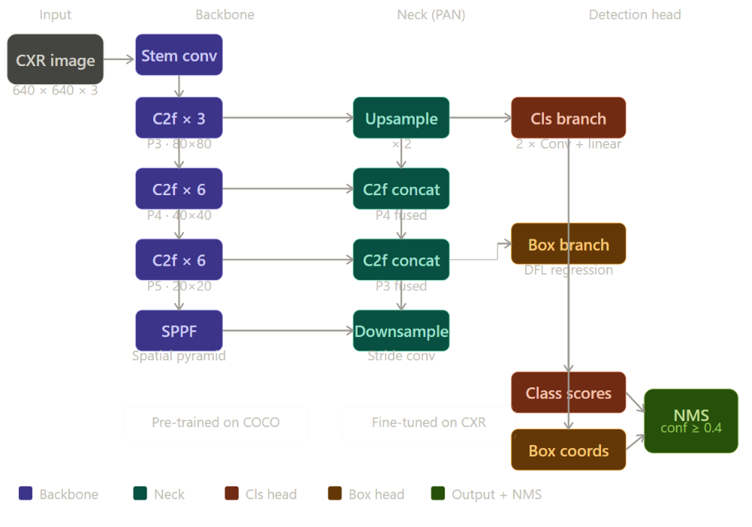
\includegraphics[width=\textwidth]{assets/yolo8_arch.png}
	\caption{YOLOv8 architecture pipeline for automated localization and classification of pulmonary abnormalities.}
	\label{fig:yolov8_architecture}
\end{figure}

\subsubsection{Mask-to-Bounding-Box Conversion}
Annotation masks for pulmonary lesions are provided as binary PNG images in which foreground pixels (intensity $> 127$) correspond to pathological regions[cite: 20, 21]. To convert these masks into YOLO-format bounding box annotations, connected component analysis is applied using external contour detection[cite: 22]. For each detected contour, an axis-aligned bounding box is computed and normalized with respect to the image dimensions, yielding center coordinates and extent values in the range $[0, 1]$[cite: 23].

Formally, for a contour with pixel-space bounding rectangle $(x, y, w, h)$ within an image of width $W$ and height $H$, the normalized YOLO representation is[cite: 24]:
\begin{equation}
	c_x = \frac{x + w/2}{W}, \quad c_y = \frac{y + h/2}{H}, \quad n_w = \frac{w}{W}, \quad n_h = \frac{h}{H} [cite: 25]
\end{equation}

Contours enclosing fewer than 5 pixels in either dimension are discarded as noise prior to annotation generation[cite: 26]. All foreground components within a given mask are assigned the class index corresponding to the image-level label (tumor or tuberculosis), since mask annotations are provided per diagnostic category[cite: 27].

\subsubsection{Dataset Preparation and Splitting}
Following bounding box conversion, the dataset is partitioned into training, validation, and test subsets using stratified random splitting[cite: 28, 29]. The default split proportions are 75\% training, 15\% validation, and 10\% test, with random seed fixed at 42 to ensure reproducibility[cite: 30]. Image files and their corresponding YOLO label files are organized into the standard YOLO directory structure, with separate image and label folders for each split[cite: 31]. A YAML configuration file is generated automatically to specify dataset paths, the number of classes, and class names, serving as the interface between the prepared dataset and the YOLOv8 training framework[cite: 32].

\subsubsection{YOLOv8 Detection Architecture}
Object detection is performed using YOLOv8, the latest generation of the You Only Look Once (YOLO) family of single-stage detectors[cite: 33, 34]. YOLOv8 follows an anchor-free design and adopts a CSPDarknet backbone for feature extraction, a Path Aggregation Network (PAN) neck for multi-scale feature fusion, and a decoupled detection head that separately predicts classification scores and bounding box offsets[cite: 35]. This design enables real-time inference while maintaining competitive localization accuracy[cite: 36].

A YOLOv8n (nano) variant is employed as the base model, pre-trained on the COCO dataset, and fine-tuned on the prepared CXR detection dataset[cite: 37]. The model is trained for 50 epochs with an input resolution of $640 \times 640$ pixels and a batch size of 16[cite: 38]. Transfer learning is leveraged by initializing all network weights from the COCO pre-trained checkpoint, with all layers unfrozen to allow domain-specific adaptation[cite: 38]. The training objective combines binary cross-entropy loss for classification, distribution focal loss (DFL) for bounding box regression, and a complete intersection-over-union (CIoU) penalty term to improve localization precision[cite: 39]:
\begin{equation}
	L = \lambda_{\text{cls}} \cdot L_{\text{cls}} + \lambda_{\text{box}} \cdot L_{\text{box}} + \lambda_{\text{dfl}} \cdot L_{\text{DFL}} [cite: 40]
\end{equation}
where $\lambda_{\text{cls}}$, $\lambda_{\text{box}}$, and $\lambda_{\text{dfl}}$ are scalar weighting coefficients that balance the contribution of each loss component during optimization[cite: 41].

After training, the best-performing checkpoint, selected based on validation mean Average Precision at IoU threshold 0.50 (mAP50), is retained for evaluation[cite: 42]. Model performance is assessed on both the held-out validation and test splits, reporting mAP50, mAP50–95, precision, and recall as primary evaluation metrics[cite: 43]. Qualitative evaluation is conducted by visually inspecting annotated predictions on test set images, examining the spatial correspondence between predicted bounding boxes and known pathological regions[cite: 44].

\begin{figure}[htbp]
	\centering
	\begin{minipage}{0.48\textwidth}
		\centering
		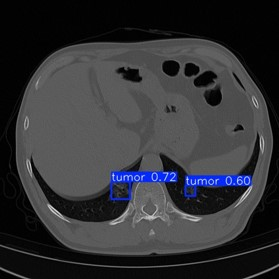
\includegraphics[width=\textwidth]{assets/lung1.jpg}
		\caption{Qualitative evaluation showing tumor localization (confidence scores 0.72 and 0.60) on an axial CT slice.}
		\label{fig:qualitative_ct_1}
	\end{minipage}\hfill
	\begin{minipage}{0.48\textwidth}
		\centering
		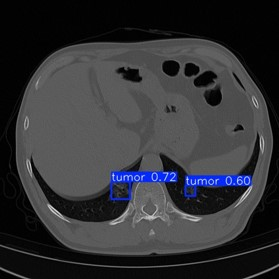
\includegraphics[width=\textwidth]{assets/lung1.jpg}
		\caption{Qualitative evaluation showing tumor localization (confidence score 0.87) on an axial CT slice.}
		\label{fig:qualitative_ct_2}
	\end{minipage}
\end{figure}

\subsection{Interpretability Considerations}
Unlike classification-only models that require post-hoc gradient visualization to identify diagnostically relevant regions, the detection framework provides explicit spatial outputs in the form of bounding boxes and associated confidence scores[cite: 45, 46]. Each prediction directly encodes the model's estimate of where a pathological region is located and how confident it is in that localization[cite: 47]. This built-in spatial explainability reduces the reliance on auxiliary interpretability methods and aligns more naturally with clinical reporting conventions, in which radiologists annotate specific anatomical regions rather than assigning image-level labels[cite: 48]. Confidence thresholding ($\tau = 0.4$) and non-maximum suppression with an IoU threshold of 0.6 are applied at inference time to filter low-quality or redundant detections, producing a concise set of high-confidence predictions per image[cite: 49].

\begin{figure}[htbp]
	\centering
	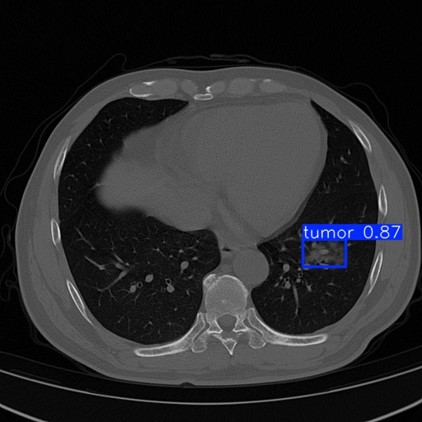
\includegraphics[width=0.6\textwidth]{assets/lung3.jpg}
	\caption{Example of an interpretable YOLO detection result on a chest CT image. The model localizes a suspected lesion using a bounding box and reports a confidence score of 0.87. Such spatial predictions provide inherent interpretability by explicitly identifying the anatomical region associated with the model's decision, reducing the need for post-hoc visualization techniques.}
	\label{fig:interpretability_example}
\end{figure}